\section{Estudio Externo -- Análisis POAM}
\label{sec:estudio_externo}

\subsection{Marco Metodológico POAM}

El Perfil de Oportunidades y Amenazas del Medio (POAM) es una metodología de análisis estratégico que permite identificar y evaluar sistemáticamente los factores externos que pueden influir en el desempeño organizacional. Este análisis se desarrolla siguiendo siete pasos metodológicos secuenciales que aseguran una evaluación integral y objetiva del entorno externo de MercadoLibre \autocite{david2017}.

La metodología POAM facilita la transformación de factores cualitativos del entorno en evaluaciones cuantitativas que permiten la priorización estratégica y la toma de decisiones fundamentadas. El análisis integra perspectivas del modelo PESTEL con evaluaciones de impacto específicas para el contexto de comercio electrónico y servicios financieros en América Latina.

\subsection{Paso 1: Unidades de Análisis}

Para el análisis POAM de MercadoLibre se han identificado seis unidades de análisis críticas que abarcan los principales factores del entorno externo:

\begin{enumerate}
\item \textbf{Entorno Económico}: Factores macroeconómicos que afectan el poder adquisitivo, tasas de interés, inflación y estabilidad monetaria en los mercados de operación.
\item \textbf{Entorno Político}: Marco regulatorio, políticas gubernamentales, estabilidad institucional y regulaciones específicas del sector fintech y e-commerce.
\item \textbf{Entorno Tecnológico}: Innovaciones tecnológicas, infraestructura digital, adopción de nuevas tecnologías y capacidades de integración sistémica.
\item \textbf{Entorno Competitivo}: Dinámica de competencia, nuevos entrantes, productos sustitutos y rivalidad en el sector.
\item \textbf{Entorno Social-Cultural}: Cambios demográficos, hábitos de consumo, preferencias culturales y adopción digital por parte de los usuarios.
\item \textbf{Entorno Ambiental}: Sostenibilidad, responsabilidad ambiental y regulaciones medioambientales.
\end{enumerate}

\subsection{Paso 2: Variables por Unidad de Análisis}

\subsubsection{Entorno Económico}
\begin{itemize}
\item Capacidad adquisitiva de la población
\item Niveles de inflación regional
\item Tasas de interés y costo de capital
\item Tipo de cambio y volatilidad monetaria
\end{itemize}

\subsubsection{Entorno Político}
\begin{itemize}
\item Aranceles de importación
\item Legislación interna de comercio electrónico
\item Regulaciones fintech y de pagos digitales
\item Estabilidad política regional
\end{itemize}

\subsubsection{Entorno Tecnológico}
\begin{itemize}
\item Nuevas tecnologías emergentes (IA, blockchain)
\item Integración con herramientas antiguas
\item Infraestructura de telecomunicaciones
\item Ciberseguridad y protección de datos
\end{itemize}

\subsubsection{Entorno Competitivo}
\begin{itemize}
\item Competencia nacional establecida
\item Competencia internacional (Amazon, Shopee)
\item Público objetivo y segmentación
\item Nuevos modelos de negocio disruptivos
\end{itemize}

\subsubsection{Entorno Social-Cultural}
\begin{itemize}
\item Envejecimiento poblacional
\item Migración de población a zonas urbanas
\item Medios de comunicación y marketing digital
\item Adopción de pagos digitales
\end{itemize}

\subsubsection{Entorno Ambiental}
\begin{itemize}
\item Políticas de sostenibilidad corporativa
\item Regulaciones ambientales
\item Logística verde y reducción de emisiones
\item Responsabilidad social empresarial
\end{itemize}

\subsection{Paso 3: Evaluación por Importancia (Relevancia)}

La evaluación de importancia se realiza en una escala de 1 a 5, donde:
\begin{itemize}
\item 1 = Muy baja importancia
\item 2 = Baja importancia  
\item 3 = Importancia media
\item 4 = Alta importancia
\item 5 = Muy alta importancia
\end{itemize}

\subsection{Paso 4: Evaluación por Impacto}

La evaluación de impacto se realiza en una escala de -3 a +3, donde:
\begin{itemize}
\item -3 = Amenaza muy alta
\item -2 = Amenaza alta
\item -1 = Amenaza media
\item 0 = Factor neutro
\item +1 = Oportunidad media
\item +2 = Oportunidad alta
\item +3 = Oportunidad muy alta
\end{itemize}

\subsection{Paso 5: Evaluación Ponderada}

La evaluación ponderada se calcula multiplicando la importancia por el impacto para cada variable analizada. Esta ponderación permite identificar los factores con mayor relevancia estratégica.

\subsection{Paso 6: Perfil de Oportunidades y Amenazas}

\begin{table}[H]
\centering
\footnotesize
\begin{tabular}{|p{2.2cm}|p{2.8cm}|c|c|c|c|c|c|c|c|c|c|}
\hline
\multirow{2}{*}{\textbf{Unidad}} & \multirow{2}{*}{\textbf{Variables}} & \multirow{2}{*}{\textbf{Imp.}} & \multirow{2}{*}{\textbf{Impacto}} & \multirow{2}{*}{\textbf{Pond.}} & \multicolumn{7}{c|}{\textbf{Escala de Evaluación}} \\
\cline{6-12}
& & & & & \textbf{-15} & \textbf{-10} & \textbf{-5} & \textbf{0} & \textbf{5} & \textbf{10} & \textbf{15} \\
\hline
\multirow{4}{*}{\makecell{Entorno\\Económico}} 
& Capacidad Adquisitiva & 4 & -2 & -8 & \multicolumn{1}{c|}{o} & \multicolumn{1}{c|}{} & \multicolumn{1}{c|}{} & \multicolumn{1}{c|}{} & \multicolumn{1}{c|}{} & \multicolumn{1}{c|}{} & \\
\cline{2-12}
& Precios & 5 & 2 & 10 & \multicolumn{1}{c|}{} & \multicolumn{1}{c|}{} & \multicolumn{1}{c|}{} & \multicolumn{1}{c|}{} & \multicolumn{1}{c|}{} & \multicolumn{1}{c|}{} & o \\
\cline{2-12}
& Tasas de Interés & 3 & 1 & 3 & \multicolumn{1}{c|}{} & \multicolumn{1}{c|}{} & \multicolumn{1}{c|}{} & \multicolumn{1}{c|}{} & \multicolumn{1}{c|}{o} & \multicolumn{1}{c|}{} & \\
\cline{2-12}
& Tipo de Cambio & 4 & -1 & -4 & \multicolumn{1}{c|}{} & \multicolumn{1}{c|}{} & \multicolumn{1}{c|}{o} & \multicolumn{1}{c|}{} & \multicolumn{1}{c|}{} & \multicolumn{1}{c|}{} & \\
\hline
\multirow{3}{*}{\makecell{Entorno\\Político}} 
& Aranceles de Importación & 3 & -1 & -3 & \multicolumn{1}{c|}{} & \multicolumn{1}{c|}{} & \multicolumn{1}{c|}{o} & \multicolumn{1}{c|}{} & \multicolumn{1}{c|}{} & \multicolumn{1}{c|}{} & \\
\cline{2-12}
& Legislación Interna & 3 & 2 & 6 & \multicolumn{1}{c|}{} & \multicolumn{1}{c|}{} & \multicolumn{1}{c|}{} & \multicolumn{1}{c|}{} & \multicolumn{1}{c|}{} & \multicolumn{1}{c|}{o} & \\
\cline{2-12}
& Regulación Fintech & 5 & 3 & 15 & \multicolumn{1}{c|}{} & \multicolumn{1}{c|}{} & \multicolumn{1}{c|}{} & \multicolumn{1}{c|}{} & \multicolumn{1}{c|}{} & \multicolumn{1}{c|}{} & o \\
\hline
\multirow{3}{*}{\makecell{Entorno\\Tecnológico}} 
& Nuevas Tecnologías & 3 & 0 & 0 & \multicolumn{1}{c|}{} & \multicolumn{1}{c|}{} & \multicolumn{1}{c|}{} & \multicolumn{1}{c|}{o} & \multicolumn{1}{c|}{} & \multicolumn{1}{c|}{} & \\
\cline{2-12}
& Integración Herramientas & 5 & 0 & 0 & \multicolumn{1}{c|}{} & \multicolumn{1}{c|}{} & \multicolumn{1}{c|}{} & \multicolumn{1}{c|}{o} & \multicolumn{1}{c|}{} & \multicolumn{1}{c|}{} & \\
\cline{2-12}
& Ciberseguridad & 5 & 1 & 5 & \multicolumn{1}{c|}{} & \multicolumn{1}{c|}{} & \multicolumn{1}{c|}{} & \multicolumn{1}{c|}{} & \multicolumn{1}{c|}{o} & \multicolumn{1}{c|}{} & \\
\hline
\multirow{4}{*}{\makecell{Entorno\\Competitivo}} 
& Competencia Nacional & 5 & 2 & 10 & \multicolumn{1}{c|}{} & \multicolumn{1}{c|}{} & \multicolumn{1}{c|}{} & \multicolumn{1}{c|}{} & \multicolumn{1}{c|}{} & \multicolumn{1}{c|}{o} & \\
\cline{2-12}
& Competencia Internacional & 3 & 1 & 3 & \multicolumn{1}{c|}{} & \multicolumn{1}{c|}{} & \multicolumn{1}{c|}{} & \multicolumn{1}{c|}{} & \multicolumn{1}{c|}{o} & \multicolumn{1}{c|}{} & \\
\cline{2-12}
& Público Objetivo & 4 & 3 & 12 & \multicolumn{1}{c|}{} & \multicolumn{1}{c|}{} & \multicolumn{1}{c|}{} & \multicolumn{1}{c|}{} & \multicolumn{1}{c|}{} & \multicolumn{1}{c|}{} & o \\
\cline{2-12}
& Modelos Disruptivos & 4 & -2 & -8 & \multicolumn{1}{c|}{o} & \multicolumn{1}{c|}{} & \multicolumn{1}{c|}{} & \multicolumn{1}{c|}{} & \multicolumn{1}{c|}{} & \multicolumn{1}{c|}{} & \\
\hline
\multirow{4}{*}{\makecell{Entorno\\Social-Cultural}} 
& Envejecimiento Poblacional & 4 & 3 & 12 & \multicolumn{1}{c|}{} & \multicolumn{1}{c|}{} & \multicolumn{1}{c|}{} & \multicolumn{1}{c|}{} & \multicolumn{1}{c|}{} & \multicolumn{1}{c|}{} & o \\
\cline{2-12}
& Migración a Zonas Urbanas & 4 & 2 & 8 & \multicolumn{1}{c|}{} & \multicolumn{1}{c|}{} & \multicolumn{1}{c|}{} & \multicolumn{1}{c|}{} & \multicolumn{1}{c|}{} & \multicolumn{1}{c|}{o} & \\
\cline{2-12}
& Medios de Comunicación & 5 & -2 & -10 & \multicolumn{1}{c|}{} & \multicolumn{1}{c|}{o} & \multicolumn{1}{c|}{} & \multicolumn{1}{c|}{} & \multicolumn{1}{c|}{} & \multicolumn{1}{c|}{} & \\
\cline{2-12}
& Adopción Digital & 5 & 3 & 15 & \multicolumn{1}{c|}{} & \multicolumn{1}{c|}{} & \multicolumn{1}{c|}{} & \multicolumn{1}{c|}{} & \multicolumn{1}{c|}{} & \multicolumn{1}{c|}{} & o \\
\hline
\multirow{2}{*}{\makecell{Entorno\\Ambiental}} 
& Sostenibilidad & 3 & 0 & 0 & \multicolumn{1}{c|}{} & \multicolumn{1}{c|}{} & \multicolumn{1}{c|}{} & \multicolumn{1}{c|}{o} & \multicolumn{1}{c|}{} & \multicolumn{1}{c|}{} & \\
\cline{2-12}
& Responsabilidad Social & 3 & 1 & 3 & \multicolumn{1}{c|}{} & \multicolumn{1}{c|}{} & \multicolumn{1}{c|}{} & \multicolumn{1}{c|}{} & \multicolumn{1}{c|}{o} & \multicolumn{1}{c|}{} & \\
\hline
\end{tabular}
\caption{Matriz POAM -- Perfil de Oportunidades y Amenazas MercadoLibre}
\label{tab:matriz_poam_completa}
\end{table}

La Tabla \ref{tab:matriz_poam_completa} presenta la evaluación detallada de todas las variables del entorno externo consideradas en el análisis POAM, permitiendo identificar las oportunidades y amenazas más relevantes para MercadoLibre \autocite{david2017}.

\subsection{Resultados Consolidados por Unidad de Análisis}

\begin{table}[H]
\centering
\begin{tabular}{|l|c|c|}
\hline
\textbf{Unidad de Análisis} & \textbf{Ponderación Total} & \textbf{Clasificación} \\
\hline
Entorno Social-Cultural & +25 & Oportunidad Significativa \\
\hline
Entorno Político & +18 & Oportunidad Significativa \\
\hline
Entorno Competitivo & +17 & Oportunidad Significativa \\
\hline
Entorno Tecnológico & +5 & Oportunidad Menor \\
\hline
Entorno Económico & +1 & Factor Neutro \\
\hline
Entorno Ambiental & +3 & Oportunidad Menor \\
\hline
\end{tabular}
\caption{Evaluación Ponderada por Unidad de Análisis -- POAM}
\label{tab:resultados_poam}
\end{table}

La Tabla \ref{tab:resultados_poam} consolida los resultados ponderados por cada unidad de análisis, mostrando que el entorno externo presenta oportunidades significativas en los aspectos social-culturales, políticos y competitivos \autocite{porter1985}.

\subsection{Paso 7: Identificación de Oportunidades y Amenazas}

\subsubsection{Principales Oportunidades Identificadas}

\begin{enumerate}
\item \textbf{Regulación Fintech Favorable (Ponderada: +15)}: Los marcos regulatorios pro-inclusión financiera en Brasil, México y Colombia facilitan la expansión de servicios de Mercado Pago y el desarrollo de nuevos productos financieros.

\item \textbf{Adopción Digital Acelerada (Ponderada: +15)}: El crecimiento en la adopción de pagos digitales y comercio electrónico en América Latina presenta oportunidades significativas de expansión de base de usuarios.

\item \textbf{Migración Urbana y Público Objetivo (Ponderada: +12)}: La concentración poblacional en zonas urbanas y la evolución demográfica favorecen la penetración de servicios digitales.

\item \textbf{Envejecimiento Poblacional (Ponderada: +12)}: El cambio demográfico crea nuevos segmentos de mercado con mayor poder adquisitivo y necesidades específicas de servicios financieros.

\item \textbf{Competencia Nacional (Ponderada: +10)}: La fragmentación de competidores locales permite oportunidades de consolidación y adquisición estratégica.
\end{enumerate}

\subsubsection{Principales Amenazas Identificadas}

\begin{enumerate}
\item \textbf{Saturación de Medios de Comunicación (Ponderada: -10)}: El incremento en costos de marketing digital y la saturación publicitaria afectan la eficiencia de adquisición de clientes.

\item \textbf{Reducción de Capacidad Adquisitiva (Ponderada: -8)}: Las presiones inflacionarias y la volatilidad económica regional impactan el poder de compra de los consumidores.

\item \textbf{Modelos de Negocio Disruptivos (Ponderada: -8)}: La entrada de competidores con modelos innovadores (como super apps asiáticas) representa amenazas al modelo tradicional de marketplace.

\item \textbf{Volatilidad Cambiaria (Ponderada: -4)}: Las fluctuaciones monetarias en mercados clave afectan la rentabilidad de operaciones transfronterizas.

\item \textbf{Aranceles de Importación (Ponderada: -3)}: Los cambios en políticas comerciales pueden impactar los costos de productos importados en la plataforma.
\end{enumerate}

\subsubsection{Estrategias de Aprovechamiento y Mitigación}

\paragraph{Para Oportunidades Principales:}
\begin{itemize}
\item Acelerar inversión en cumplimiento regulatorio y obtención de licencias fintech
\item Desarrollar productos específicos para segmentos demográficos emergentes
\item Implementar estrategias de adquisición de competidores locales fragmentados
\item Expandir servicios de inclusión financiera aprovechando marcos regulatorios favorables
\end{itemize}

\paragraph{Para Amenazas Principales:}
\begin{itemize}
\item Diversificar canales de marketing y optimizar eficiencia de CAC
\item Implementar estrategias de pricing dinámico sensible a condiciones económicas
\item Desarrollar capacidades de innovación interna para anticipar disrupciones
\item Establecer coberturas financieras para mitigar riesgo cambiario
\end{itemize}

\subsection{Cuadro de Mando Integral}

El Cuadro de Mando Integral (Balanced Scorecard) representa una herramienta estratégica fundamental que permite traducir la visión y estrategia de MercadoLibre en un conjunto coherente de indicadores de desempeño. Esta metodología facilita la alineación organizacional y el seguimiento sistemático del progreso hacia los objetivos estratégicos, integrando perspectivas financieras y no financieras en un marco de gestión integral.

\begin{table}[H]
    \centering
    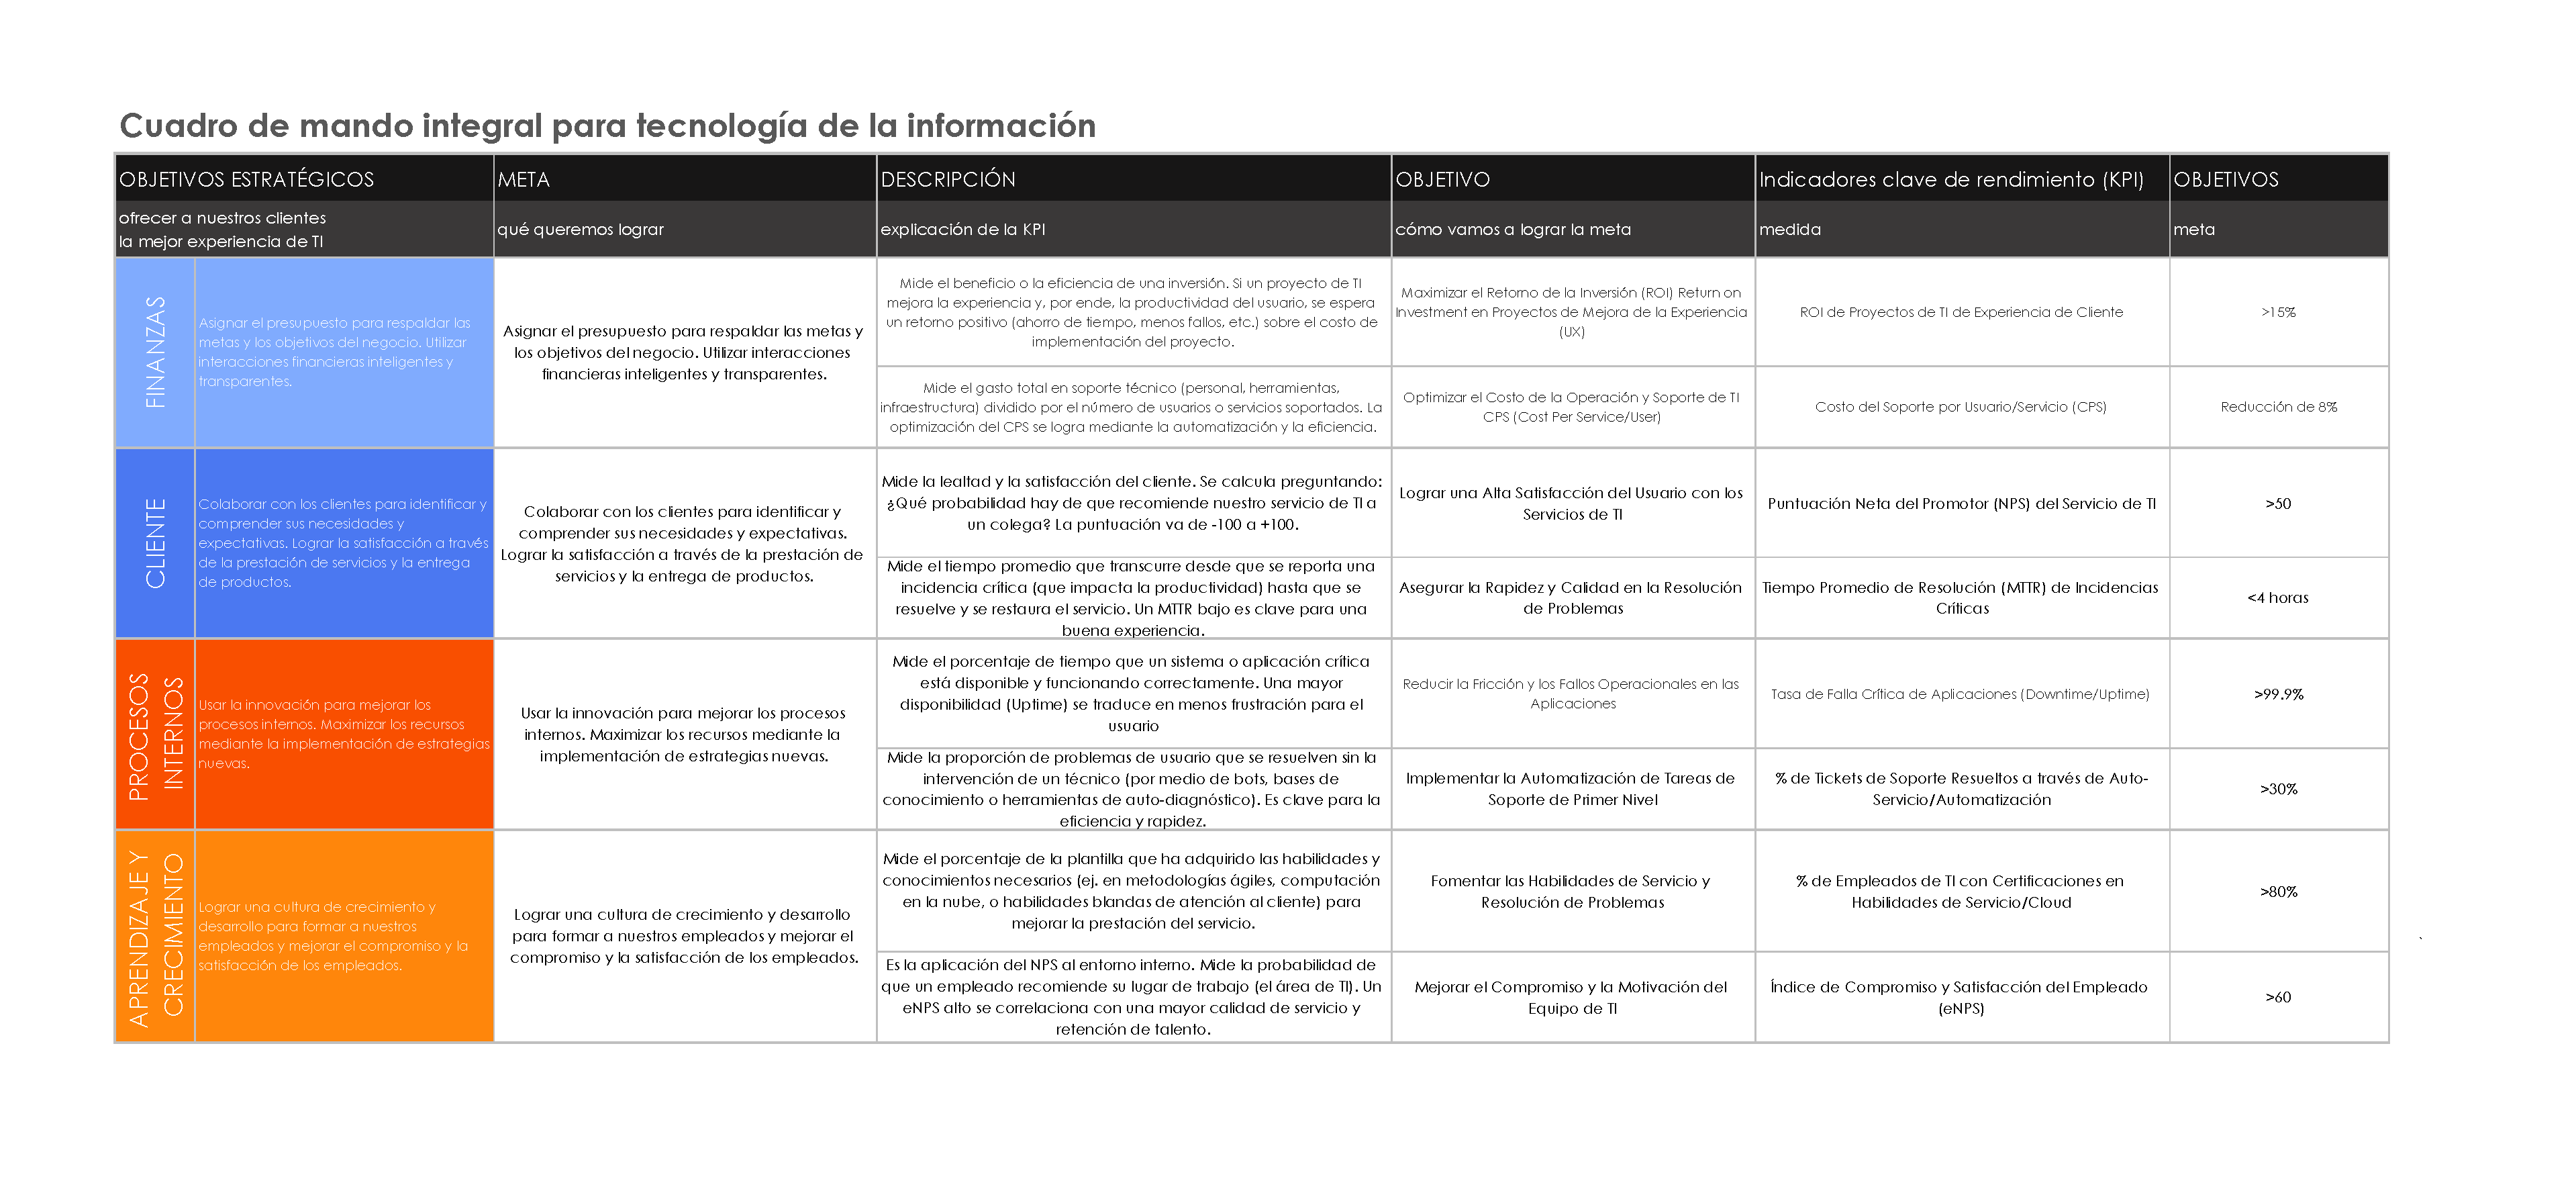
\includegraphics[width=\linewidth, height=0.8\textheight, keepaspectratio]{sections/Cuadro_Mando_Mercado_Libre.pdf}
    \caption{Cuadro de Mando Integral MercadoLibre}
    \label{tab:cuadro_mando_integral}
\end{table}

La Tabla \ref{tab:cuadro_mando_integral} presenta el Cuadro de Mando Integral diseñado específicamente para MercadoLibre, estructurado en las cuatro perspectivas clásicas del modelo: Financiera, Cliente, Procesos Internos, y Aprendizaje y Crecimiento. Este marco estratégico permite monitorear tanto los resultados operativos como los inductores de valor futuro, garantizando una gestión equilibrada entre objetivos de corto y largo plazo.

\subsection{Conclusiones del Análisis POAM}

El análisis POAM revela un entorno externo predominantemente favorable para MercadoLibre, con oportunidades significativas concentradas en regulación fintech y adopción digital. Las principales amenazas se relacionan con presiones de marketing y volatilidad económica, factores que requieren estrategias de mitigación específicas pero no comprometen la viabilidad del modelo de negocio.

La evaluación ponderada indica que los factores positivos superan significativamente a los negativos, sugiriendo un contexto estratégico propicio para la expansión y consolidación de la posición competitiva en el mercado latinoamericano de comercio electrónico y servicios financieros \autocite{porter1985}.
